\section{Image experiments and the limits of transfer}
\label{sec:real}\label{sec:real-data}\label{sec:spectral-predictor}

\paragraph{Setup.}
For each dataset (CelebA and CIFAR-10 at $32\times32$) and each $\dlat$ we train a convolutional VAE on the full training split, freeze it, and train a depth-five MLP score model (hidden width 1024, sinusoidal time features, so parameter count is roughly constant across widths) on the encoder means of a farthest-first diverse subset of 1k training images, with SGD (learning rate $10^{-3}$, momentum $0.8$), batch size 512, 5M steps and five seeds (\cref{app:methods}). Memorization is the pixel-space nearest-neighbour ratio of 10k decoded samples against the 1k subset, evaluated every 100k steps; FID uses the same reference. A narrow VAE erases sample identity before the score model can copy it: the smallest width whose own reconstructions pass the memorization test on $95\%$ of the subset is $\approx70$ on CelebA and $\approx140$ on CIFAR-10, and only widths above this identity threshold test the width effect.

\paragraph{Result.}
Post-identity-threshold width comparisons show longer times to memorization. The mean first evaluation step at which $5\%$ of samples are memorized rises from $0.32$M at $\dlat=80$ to $1.16$M at $\dlat=200$ on CelebA ($3.6\times$), and from $1.04$M at $\dlat=160$ to $1.50$M at $\dlat=240$ on CIFAR-10 ($1.4\times$; \cref{tab:hitting-times-real}). Both comparisons start above the identity threshold; the CIFAR-10 trend is not strictly monotone. The final fraction after 5M steps peaks near the identity threshold ($\dlat=70$--$80$ on CelebA) and falls by roughly half by $\dlat=200$; on CIFAR-10 it stays high through $\dlat=100$--$160$ and then declines. FID improves as the bottleneck is relieved, is best at intermediate widths, and worsens again at the widest latents (CelebA: $38.9$ at $\dlat=140$ to $47$--$50$ at $\dlat=160$--$200$), so width trades quality against memorization rather than buying both (\cref{fig:real-main}).

\begin{figure}[t]
  \centering
  \begin{subfigure}{0.48\linewidth}
    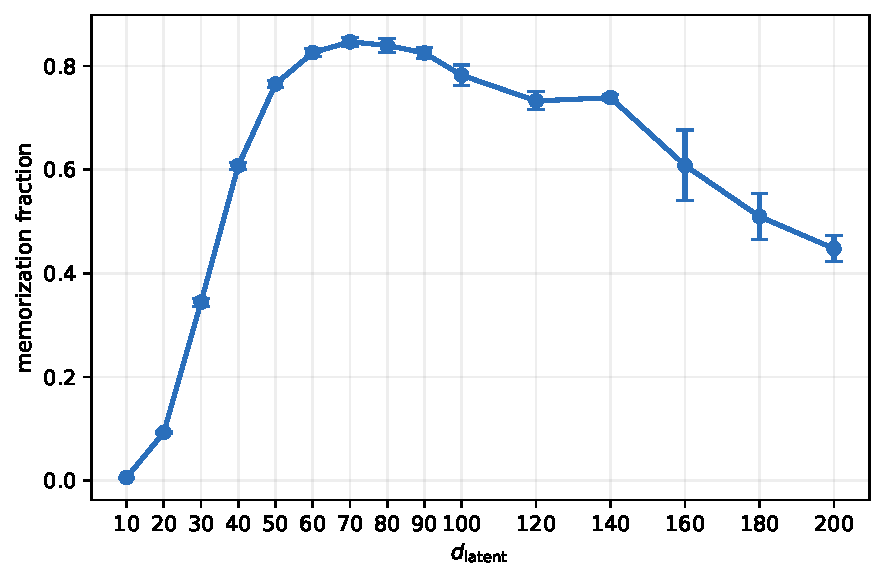
\includegraphics[width=\linewidth]{figures/celeba_final_mem_vs_d.pdf}
  \end{subfigure}\hfill
  \begin{subfigure}{0.48\linewidth}
    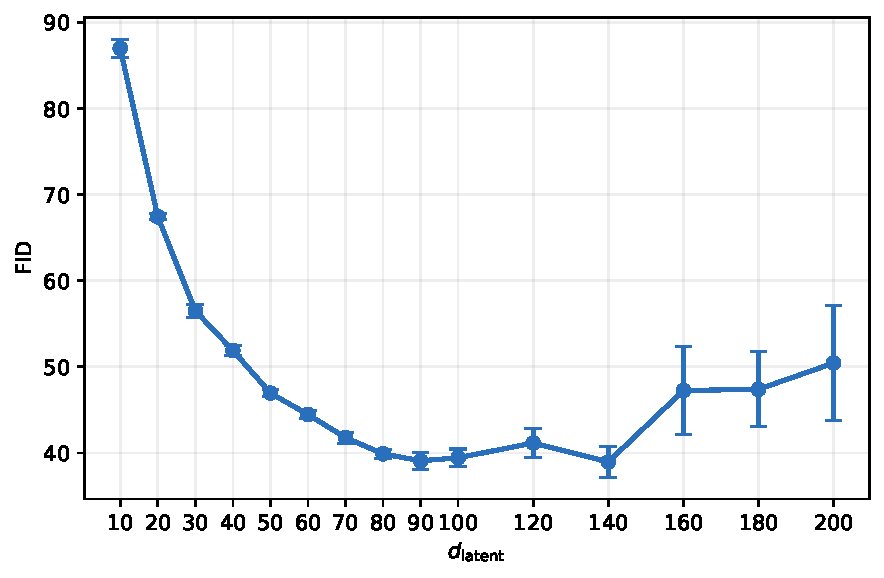
\includegraphics[width=\linewidth]{figures/celeba_final_fid_vs_d.pdf}
  \end{subfigure}
  \begin{subfigure}{0.48\linewidth}
    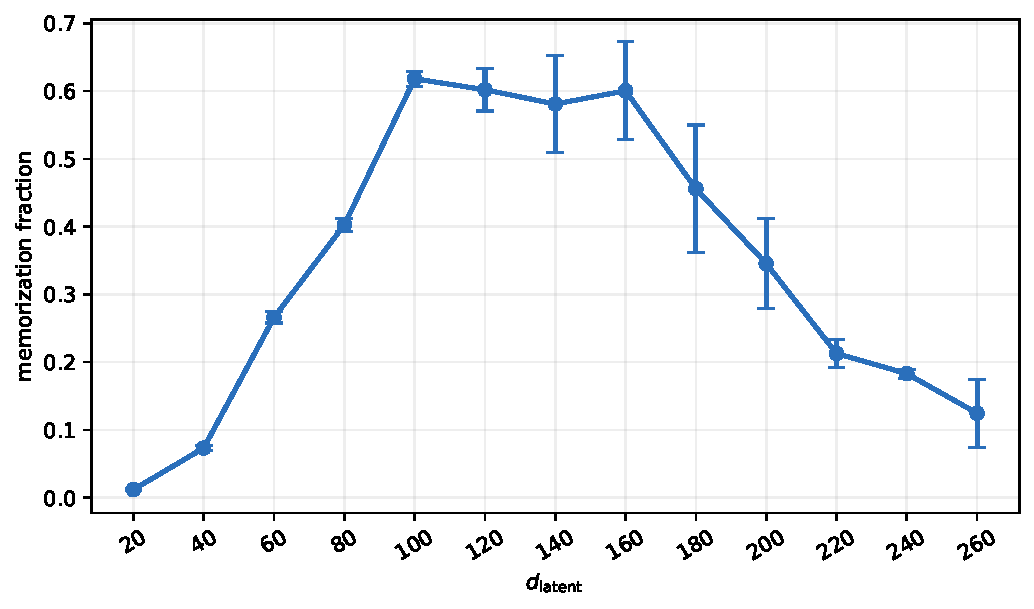
\includegraphics[width=\linewidth]{figures/cifar10_final_mem_vs_d.pdf}
  \end{subfigure}\hfill
  \begin{subfigure}{0.48\linewidth}
    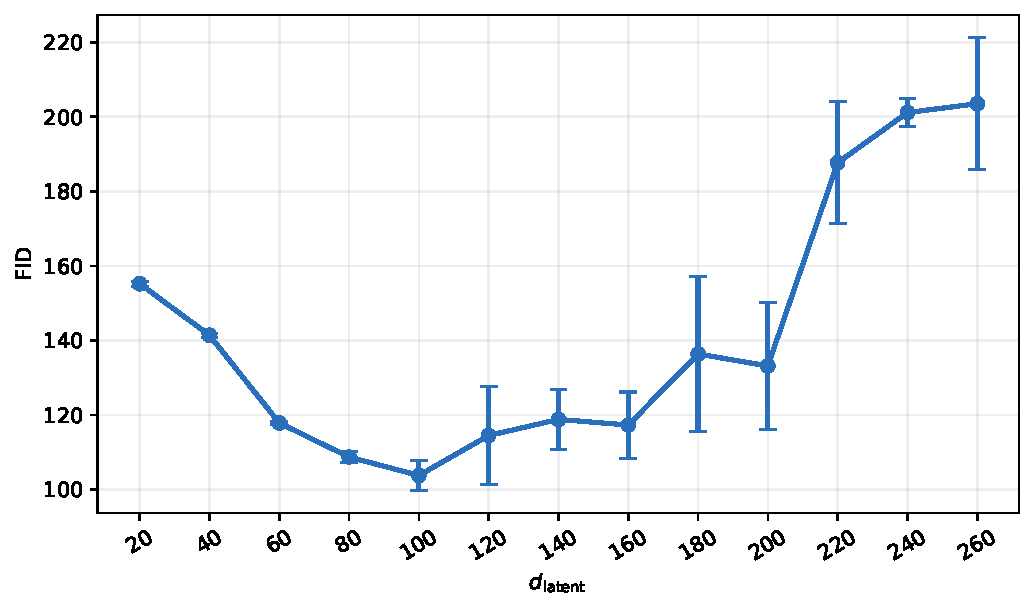
\includegraphics[width=\linewidth]{figures/cifar10_final_fid_vs_d.pdf}
  \end{subfigure}
  \caption{Final memorized fraction (left) and FID (right) after 5M steps against latent width, CelebA (top) and CIFAR-10 (bottom); five-seed means with $95\%$ confidence intervals. Below the identity threshold the VAE hides memorization; above it, memorization falls with width while FID first improves and then worsens.}
  \label{fig:real-main}
\end{figure}

\paragraph{What carries over from the frozen-feature model.}
The mechanism of \cref{sec:theory} acts through the operating point $q_d=\mathrm{tr}\,M_t/\dlat$, the pre-activation variance of the isotropic frozen-feature surrogate. On real latents the nominal width is not the axis the model sees. Beyond $\dlat\sim140$ on CelebA and $\sim160$ on CIFAR-10 the coordinates the VAE adds are posterior-collapsed: their eigenvalues sit at the diffusion floor $\Delta_t$ (at least $15\%$ of coordinates for CelebA $\dlat\ge180$), the trace of the latent covariance is flat ($252.5$, $255.2$, $260.4$ at $\dlat=160,180,200$), and the effective dimension saturates ($89.5$, $90.3$, $87.9$). The surrogate summarizes this change through $q_d$, which falls from $1.473$ to $1.247$ over CelebA $160\to200$. Reading the surrogate at these values gives the right sign, longer hitting times and smaller final fractions, and accounts for $0.55$--$0.82$ of the log-slowdown of CelebA hitting times over $160\to200$ and $0.46$ on CIFAR-10 over $160\to260$, but only $0.28$ and $0.15$ of the log-decline of the final fractions (\cref{app:theory}). The remainder is outside the surrogate.

\paragraph{What does not.}
Two boundaries. (i) The mechanism is verified in the random-feature network but not shown to be what delays memorization in trained networks. In the synthetic MLPs of \cref{sec:phenomenon}, the first-layer mean-square pre-activation $q_{\rm M}$ is similar at 50k steps ($0.71$ at $\dlat=5$, $0.68$ at $\dlat=40$); it separates later, growing with memorization at small width: $q_{\rm M}(40)/q_{\rm M}(5)=0.96,\,0.70,\,0.47,\,0.30$ at $0.05$M, $0.25$M, $1$M and $5$M steps (five seeds; protocol in \cref{app:mlp-preactivation}), while the memorized fraction at $\dlat=5$ rises from $0.6\%$ to $29.9\%$. These measurements do not establish a width-set difference in $q_{\rm M}$ preceding memorization. A candidate explanation consistent with the same data sits on the target side: the per-coordinate gap between the empirical and population scores grows $3.6\times$ ($3.7$ to $13.2$) from $\dlat=5$ to $40$, so a memorizing network must fit a sharper target and grow its first-layer scale to do so. We state this as a hypothesis. (ii) The effect is not architecture-independent. In a CelebA pilot with a spatial $4\times4\times\dlat$ VAE and a DiT-style score network, memorization rises with channel count, from about $22\%$ at $\dlat=5$ to roughly $48\%$ by $\dlat=8$--$10$, and the broad sweep shows no clean decline at large widths (\cref{fig:app-spatial-dit-summary,fig:app-spatial-dit-lowd}). Channel count there changes sixteen coordinates at once together with their spatial covariance, so it is not the same control; but the fixed-width MLP result cannot be assumed to transfer.

\paragraph{Predicting onset from the frozen latent spectrum.}\label{sec:predictor}
The appendix (\cref{app:theory}) turns the sample-mode eigenvalue of the frozen VAE latent spectrum into a one-constant clock for the memorization onset, $\tau_f(\dlat)=C\nsamp/g(q_d,1-\Delta_t/q_d)$ with $q_d=\operatorname{tr}M_t/\dlat$. Fit on all widths but one and evaluated on the held-out width, its log error is $0.41$ on CelebA ($\dlat\ge50$) and $0.15$ on CIFAR-10 ($\dlat\ge60$), comparable to the seven-parameter in-sample fit of the released predictor ($0.34$ and $0.15$); but a clock that depends on $\dlat$ alone reaches $0.13$ on CelebA, the fitted constant differs by $2\times$ between datasets, and over the broader CelebA $50\to200$ sweep it captures only $1.78\times$ of the $3.9\times$ slowdown. These diagnostic fits include widths below the identity threshold. We therefore report it as a diagnostic, not a contribution.
